% move all configuration stuff into one file so we can focus on the content
\documentclass[aspectratio=169,hyperref={pdfpagelabels=false,colorlinks=true,linkcolor=white,urlcolor=lightblue},xcolor={table},t]{beamer}

%%%%%%%%%%%%%%%%%%%%%%%%%%%%%%%%%%%%%%%%%%%%%%%%%%%%%%%%%%%%%%%%%%%%%%%%%%%%%%%%%%
%%%%%%%%%%%%%%%%%%%%%%%%%%%%%%%%%%%%%%%%%%%%%%%%%%%%%%%%%%%%%%%%%%%%%%%%%%%%%%%%%%
% packages
\usepackage{pict2e}
\usepackage{epic}
\usepackage{amsmath,amsfonts,amssymb}
\usepackage{units}
\usepackage{fancybox}
\usepackage[absolute,overlay]{textpos} 
%\usepackage[table]{xcolor}
\usepackage{animate}
\usepackage{gensymb}
%\usepackage{graphicx}
%\usepackage{longtable}
\usepackage{multirow}
\usepackage{silence}
\usepackage{tikz}
\usepackage[backend=bibtex,style=ieee]{biblatex}
\AtEveryCitekey{\iffootnote{\tiny}{}}
%\addbibresource{include/references}



% fontsize
\let\Tiny=\tiny

%%%%%%%%%%%%%%%%%%%%%%%%%%%%%%%%%%%%%%%%%%%%%%%%%%%%%%%%%%%%%%%%%%%%%%%%%%%%%%%%%%
%%%%%%%%%%%%%%%%%%%%%%%%%%%%%%%%%%%%%%%%%%%%%%%%%%%%%%%%%%%%%%%%%%%%%%%%%%%%%%%%%%
% warnings
\pdfsuppresswarningpagegroup=1
\WarningFilter{biblatex}{Patching footnotes failed}
\WarningFilter{latexfont}{Font shape}
\WarningFilter{latexfont}{Some font shapes}
\WarningFilter{gensymb}{Not defining}


%%%%%%%%%%%%%%%%%%%%%%%%%%%%%%%%%%%%%%%%%%%%%%%%%%%%%%%%%%%%%%%%%%%%%%%%%%%%%%%%%%
%%%%%%%%%%%%%%%%%%%%%%%%%%%%%%%%%%%%%%%%%%%%%%%%%%%%%%%%%%%%%%%%%%%%%%%%%%%%%%%%%%
% theme & layout
\usetheme{Frankfurt}
\useinnertheme{rectangles}


%%%%%%%%%%%%%%%%%%%%%%%%%%%%%%%%%%%%%%%%%%%%%%%%%%%%%%%%%%%%%%%%%%%%%%%%%%%%%%%%%%
\setbeamertemplate{frametitle}[default][colsep=-4bp,rounded=false,shadow=false]
\setbeamertemplate{frametitle}
{%
    \nointerlineskip%
    %\vskip-0.5ex
    \begin{beamercolorbox}[wd=\paperwidth,ht=3.5ex,dp=0.6ex]{frametitle}
        \hspace*{1.3ex}\insertframetitle%
        
        \hspace*{1.3ex}\small\insertframesubtitle%
    \end{beamercolorbox}%
    \begin{textblock*}{100mm}(13.75cm,1cm)
        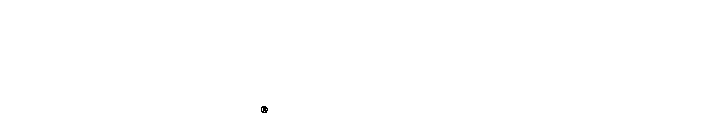
\includegraphics[height=.4cm,keepaspectratio]{../shared/Logo_GTCMT_white}
    \end{textblock*}
}


%%%%%%%%%%%%%%%%%%%%%%%%%%%%%%%%%%%%%%%%%%%%%%%%%%%%%%%%%%%%%%%%%%%%%%%%%%%%%%%%%%
\setbeamertemplate{title page}[default][colsep=-4bp,rounded=false,shadow=false]
\setbeamertemplate{title page}
{
    %\begin{textblock*}{100mm}(15cm,.51cm)
            %\href{https://github.com/alexanderlerch/ACA-Slides/blob/2nd_edition/\jobname.pdf}{\includegraphics[height=.5cm,keepaspectratio]{graph/Logo_github}}\hspace*{2ex}
    %\end{textblock*}
    %\begin{textblock*}{100mm}(15cm,1.3cm)
            %\href{\IEEELink}{\includegraphics[height=.5cm,keepaspectratio]{graph/icon/book}}\hspace*{2ex}
    %\end{textblock*}
    \vskip-10ex
    \begin{beamercolorbox}[wd=\paperwidth,ht=.7\paperheight,dp=0.6ex]{frametitle} %35ex
        %\begin{flushright}
            %\href{http://www.gtcmt.gatech.edu}{
\includegraphics[height=.8cm,keepaspectratio]{graph/Logo_GTCMT_black}}\hspace*{2ex}
        %\end{flushright}
        
        \hspace*{1.8ex}\LARGE\inserttitle%
        
        \vspace*{.5ex}
        
        \hspace*{1.3ex}\small\insertsubtitle%
        
        \vspace*{.5ex}
    \end{beamercolorbox}%
    \nointerlineskip%
    \begin{beamercolorbox}[wd=\paperwidth,ht=.4\paperheight,dp=0.6ex]{page number in head/foot}
        %\vspace*{-.5ex}
        \hspace*{1.7ex}\small\insertauthor%
        
        %\hspace*{1.7ex}\small }%
        
        \vspace*{12ex}
        \vfill
        \begin{flushright}
            \href{http://www.gtcmt.gatech.edu}{
\includegraphics[height=.5cm,keepaspectratio]{../shared/Logo_GTCMT_black}}\hspace*{2ex}
        \end{flushright}
    \end{beamercolorbox}%
}


%%%%%%%%%%%%%%%%%%%%%%%%%%%%%%%%%%%%%%%%%%%%%%%%%%%%%%%%%%%%%%%%%%%%%%%%%%%%%%%%%%
%\makeatother
\setbeamertemplate{footline}
{
  \leavevmode%
  \hbox{%
  \begin{beamercolorbox}[wd=.5\paperwidth,ht=2.25ex,dp=1ex,left,leftskip=1ex]{page number in head/foot}%
    \insertsubtitle
  \end{beamercolorbox}%
  \begin{beamercolorbox}[wd=.5\paperwidth,ht=2.25ex,dp=1ex,right,rightskip=1ex]{page number in head/foot}%
    \hfill
    \insertframenumber{} / \inserttotalframenumber
  \end{beamercolorbox}}%
  \vskip0pt%
}
%\makeatletter


%%%%%%%%%%%%%%%%%%%%%%%%%%%%%%%%%%%%%%%%%%%%%%%%%%%%%%%%%%%%%%%%%%%%%%%%%%%%%%%%%%
\beamertemplatenavigationsymbolsempty
\setbeamertemplate{navigation symbols}{}
\setbeamertemplate{blocks}[default]%[rounded=false,shadow=false]
\setbeamertemplate{itemize item}[square]
\setbeamertemplate{itemize subitem}[circle]
\setbeamertemplate{itemize subsubitem}[triangle]
\setbeamertemplate{enumerate item}[square]
\setbeamertemplate{enumerate subitem}[circle]
\setbeamertemplate{enumerate subsubitem}[circle]


%%%%%%%%%%%%%%%%%%%%%%%%%%%%%%%%%%%%%%%%%%%%%%%%%%%%%%%%%%%%%%%%%%%%%%%%%%%%%%%%%%
% colors
\setbeamercolor{structure}{fg=darkgray}
\setbeamercovered{transparent} %invisible
\setbeamercolor{bibliography entry author}{fg=black}
\setbeamercolor*{bibliography entry title}{fg=black}
\setbeamercolor*{bibliography entry note}{fg=black}
\setbeamercolor{frametitle}{fg=black}
\setbeamercolor{title}{fg=white}
\setbeamercolor{subtitle}{fg=white}
\setbeamercolor{frametitle}{fg=white}
\setbeamercolor{framesubtitle}{fg=white}
\setbeamercolor{mini frame}{fg=white, bg=black}
\setbeamercolor{section in head/foot}{fg=white, bg=darkgray}
\setbeamercolor{page number in head/foot}{fg=black, bg=gtgold}
\setbeamercolor{item projected}{fg=white, bg=black}

%---------------------------------------------------------------------------------

%%%%%%%%%%%%%%%%%%%%%%%%%%%%%%%%%%%%%%%%%%%%%%%%%%%%%%%%%%%%%%%%%%%%%%%%%%%%%%%%%%
%%%%%%%%%%%%%%%%%%%%%%%%%%%%%%%%%%%%%%%%%%%%%%%%%%%%%%%%%%%%%%%%%%%%%%%%%%%%%%%%%%
% title information
\title[]{MUSI6202: Digital Signal Processing for Music}   
\author[alexander lerch]{alexander lerch} 
%\institute{~}
%\date[Alexander Lerch]{}
%\titlegraphic{\vspace{-16mm}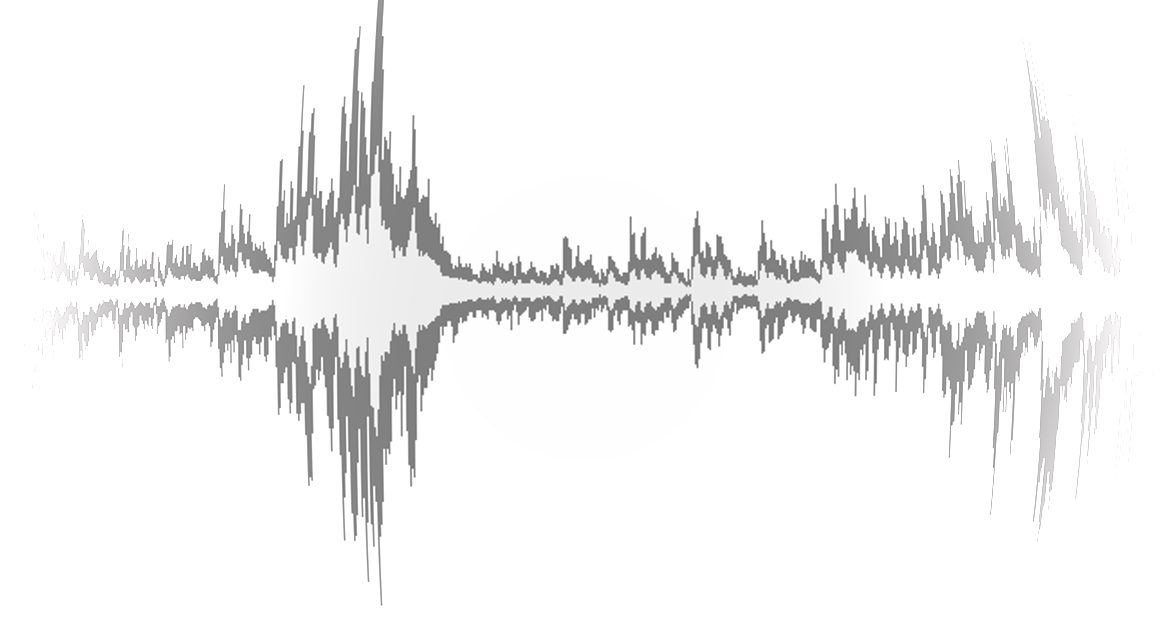
\includegraphics[width=\textwidth,height=3cm]{title}}

%%%%%%%%%%%%%%%%%%%%%%%%%%%%%%%%%%%%%%%%%%%%%%%%%%%%%%%%%%%%%%%%%%%%%%%%%%%%%%%%%%
%%%%%%%%%%%%%%%%%%%%%%%%%%%%%%%%%%%%%%%%%%%%%%%%%%%%%%%%%%%%%%%%%%%%%%%%%%%%%%%%%%
% colors
\definecolor{gtgold}{rgb}{.914, .664, 0} %0e7eed {rgb}{0.88,0.66,1,0.06} [234, 170, 0]/256 %96caff
\definecolor{darkgray}{rgb}{.15, .15, .15}
\definecolor{lightblue}{HTML}{0e7eed}
\definecolor{highlight}{rgb}{0, 0, 1} %_less!40

%%%%%%%%%%%%%%%%%%%%%%%%%%%%%%%%%%%%%%%%%%%%%%%%%%%%%%%%%%%%%%%%%%%%%%%%%%%%%%%%%%
%%%%%%%%%%%%%%%%%%%%%%%%%%%%%%%%%%%%%%%%%%%%%%%%%%%%%%%%%%%%%%%%%%%%%%%%%%%%%%%%%%
% relative paths
\graphicspath{{../graph/}}


%%%%%%%%%%%%%%%%%%%%%%%%%%%%%%%%%%%%%%%%%%%%%%%%%%%%%%%%%%%%%%%%%%%%%%%%%%%%%%%%%%
%%%%%%%%%%%%%%%%%%%%%%%%%%%%%%%%%%%%%%%%%%%%%%%%%%%%%%%%%%%%%%%%%%%%%%%%%%%%%%%%%%
% units
\setlength{\unitlength}{1mm}

%%%%%%%%%%%%%%%%%%%%%%%%%%%%%%%%%%%%%%%%%%%%%%%%%%%%%%%%%%%%%%%%%%%%%%%%%%%%%%%%%%
%%%%%%%%%%%%%%%%%%%%%%%%%%%%%%%%%%%%%%%%%%%%%%%%%%%%%%%%%%%%%%%%%%%%%%%%%%%%%%%%%%
% math
\DeclareMathOperator*{\argmax}{argmax}
\DeclareMathOperator*{\argmin}{argmin}
\DeclareMathOperator*{\atan}{atan}
\DeclareMathOperator*{\arcsinh}{arcsinh}
\DeclareMathOperator*{\sign}{sign}
\DeclareMathOperator*{\tcdf}{tcdf}
\DeclareMathOperator*{\si}{sinc}
\DeclareMathOperator*{\princarg}{princarg}
\DeclareMathOperator*{\arccosh}{arccosh}
\DeclareMathOperator*{\hwr}{HWR}
\DeclareMathOperator*{\flip}{flip}
\DeclareMathOperator*{\sinc}{sinc}
\DeclareMathOperator*{\floor}{floor}
\newcommand{\e}{{e}}
\newcommand{\jom}{\mathrm{j}\omega}
\newcommand{\jOm}{\mathrm{j}\Omega}
\newcommand   {\mat}[1]    		{\boldsymbol{\uppercase{#1}}}		%bold
\renewcommand {\vec}[1]    		{\boldsymbol{\lowercase{#1}}}		%bold

%%%%%%%%%%%%%%%%%%%%%%%%%%%%%%%%%%%%%%%%%%%%%%%%%%%%%%%%%%%%%%%%%%%%%%%%%%%%%%%%%%
%%%%%%%%%%%%%%%%%%%%%%%%%%%%%%%%%%%%%%%%%%%%%%%%%%%%%%%%%%%%%%%%%%%%%%%%%%%%%%%%%%
% media9
\newcommand{\includeaudio}[1]{
\href{run:audio/#1.mp3}{
\includegraphics[width=5mm, height=5mm]{graph/SpeakerIcon}}}

\newcommand{\includeanimation}[4]{{\begin{center}
                        \animategraphics[autoplay,loop,scale=.7]{#4}{animation/#1-}{#2}{#3}        
                        \end{center}
                        \addreference{matlab source: \href{https://github.com/alexanderlerch/ACA-Plots/blob/master/matlab/animate#1.m}{matlab/animate#1.m}}}
                        \inserticon{video}}
                        
%%%%%%%%%%%%%%%%%%%%%%%%%%%%%%%%%%%%%%%%%%%%%%%%%%%%%%%%%%%%%%%%%%%%%%%%%%%%%%%%%%
%%%%%%%%%%%%%%%%%%%%%%%%%%%%%%%%%%%%%%%%%%%%%%%%%%%%%%%%%%%%%%%%%%%%%%%%%%%%%%%%%%
% other commands
\newcommand{\question}[1]{%\vspace{-4mm}
                          \setbeamercovered{invisible}
                          \begin{columns}[T]
                            \column{.9\textwidth}
                                \textbf{#1}
                            \column{.1\textwidth}
                                \vspace{-8mm}
                                \begin{flushright}
                                     
\includegraphics[width=.9\columnwidth]{graph/question_mark}
                                \end{flushright}
                                \vspace{6mm}
                          \end{columns}\pause\vspace{-12mm}}

\newcommand{\toremember}[1]{
                        \inserticon{lightbulb}
                        }

\newcommand{\matlabexercise}[1]{%\vspace{-4mm}
                          \setbeamercovered{invisible}
                          \begin{columns}[T]
                            \column{.8\textwidth}
                                \textbf{matlab exercise}: #1
                            \column{.2\textwidth}
                                \begin{flushright}
                                     \includegraphics[scale=.5]{graph/logo_matlab}
                                \end{flushright}
                                %\vspace{6mm}
                          \end{columns}}

\newcommand{\addreference}[1]{  
                  
                    \begin{textblock*}{\baselineskip }(.98\paperwidth,.5\textheight) %(1.15\textwidth,.4\textheight)
                         \begin{minipage}[b][.5\paperheight][b]{1cm}%
                            \vfill%
                             \rotatebox{90}{\tiny {#1}}
                        \end{minipage}
                   \end{textblock*}
                    }
                    
\newcommand{\figwithmatlab}[1]{
                    \begin{figure}
                        \centering
                        \includegraphics[scale=.7]{#1}
                        %\label{fig:#1}
                    \end{figure}
                    
                    \addreference{matlab source: \href{https://github.com/alexanderlerch/MUSI-6202/blob/main/matlab/plot#1.m}{plot#1.m}}}
\newcommand{\figwithref}[2]{
                    \begin{figure}
                        \centering
                        \includegraphics[scale=.7]{#1}
                        \label{fig:#1}
                    \end{figure}
                    
                    \addreference{#2}}  
                                    
\newcommand{\inserticon}[1]{
                    \begin{textblock*}{100mm}(14.5cm,7.5cm)
                        \includegraphics[height=.8cm,keepaspectratio]{graph/#1}
                    \end{textblock*}}            

%%%%%%%%%%%%%%%%%%%%%%%%%%%%%%%%%%%%%%%%%%%%%%%%%%%%%%%%%%%%%%%%%%%%%%%%%%%%%%%%%%
%%%%%%%%%%%%%%%%%%%%%%%%%%%%%%%%%%%%%%%%%%%%%%%%%%%%%%%%%%%%%%%%%%%%%%%%%%%%%%%%%%
% counters
\newcounter{i}
\newcounter{j}
\newcounter{iXOffset}
\newcounter{iYOffset}
\newcounter{iXBlockSize}
\newcounter{iYBlockSize}
\newcounter{iYBlockSizeDiv2}
\newcounter{iXBlockSizeDiv2}
\newcounter{iDistance}

\newcommand{\IEEELink}{https://ieeexplore.ieee.org/servlet/opac?bknumber=9965970}

\addbibresource{../shared/references}



\subtitle{Part 20: Reverb}

%%%%%%%%%%%%%%%%%%%%%%%%%%%%%%%%%%%%%%%%%%%%%%%%%%%%%%%%%%%%%%%%%%%%%%%%%%%%
\begin{document}
    % generate title page
	\title[]{Digital Signal Processing for Music}   
\author[alexander lerch]{alexander lerch} 
%\institute{~}
%\date[Alexander Lerch]{}
\titlegraphic{\vspace{-16mm}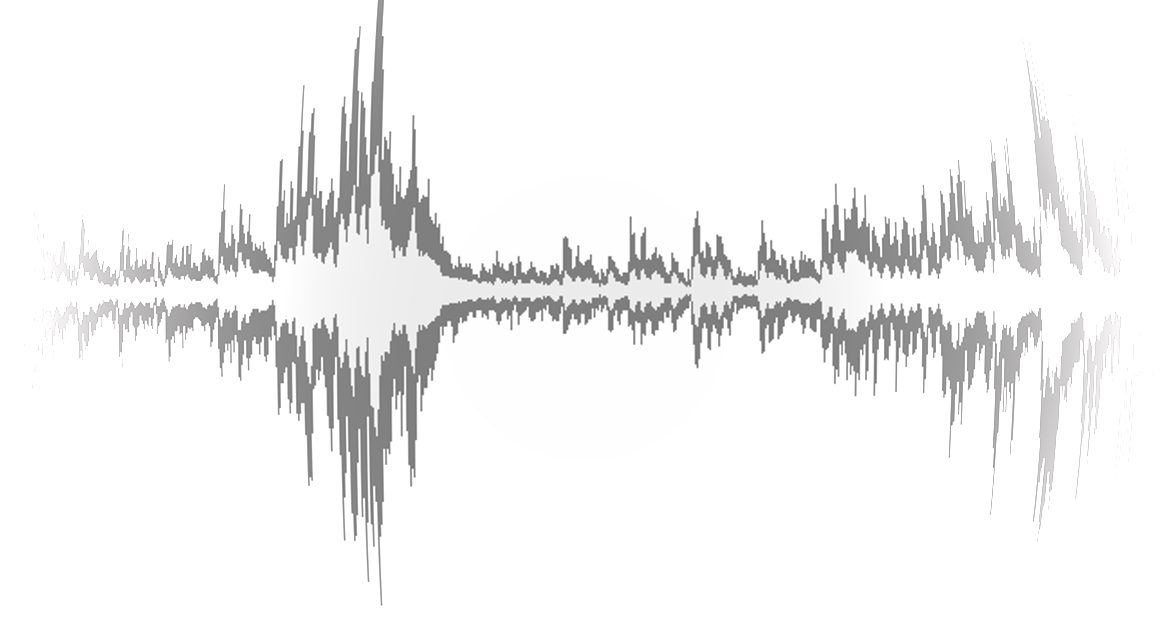
\includegraphics[width=\textwidth,height=3cm]{title}}


\begin{frame}
    \titlepage
    %\vspace{-5mm}
    \begin{flushright}
        \href{http://www.gtcmt.gatech.edu}{
\includegraphics[height=.8cm,keepaspectratio]{../shared/Logo_GTCMT_black}}
    \end{flushright}
\end{frame}


\section{intro}
\begin{frame}{artificial reverberation}{introduction}
	\begin{itemize}
		\item	\textbf{idea}:\\
				\begin{itemize}
					\item	artificially generate the impression of envelopment and reverberation
					\item	possibly allow to modify specific characteristics of the ``modeled'' room
				\end{itemize}
		\pause
        \bigskip
		\item	\textbf{approaches}
			\begin{itemize}
				\item	(digital) parametric reverberation (predecessors: spring, plate, room, \ldots)
				\item	fast convolution
			\end{itemize}	
	\end{itemize}
\end{frame}

\section{room acoustics}
\begin{frame}{artificial reverberation}{room impulse response}
	\vspace{-3mm}\begin{figure}
		\centerline{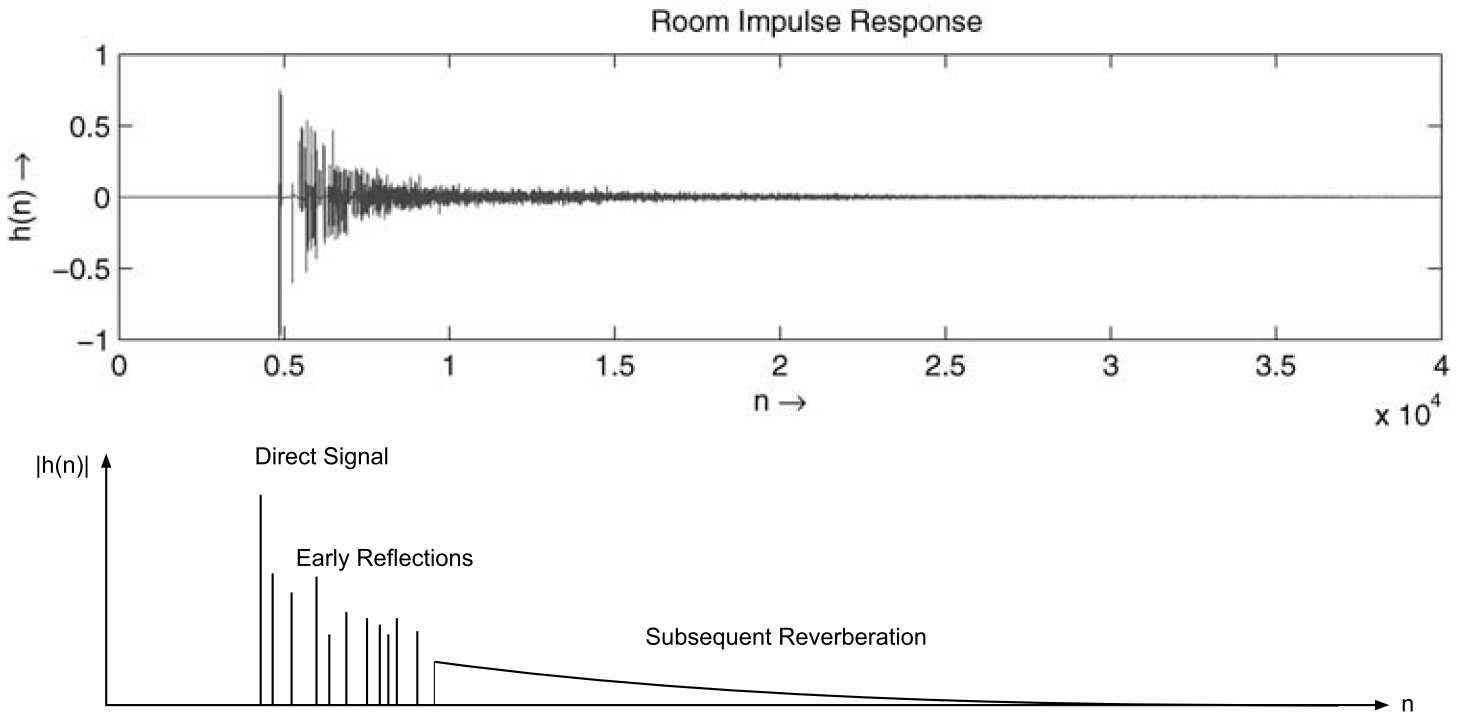
\includegraphics[scale=.28]{graph/IR}}
	\end{figure}
    \phantom{\footfullcite{zolzer_digital_2008}}
\end{frame}

\begin{frame}{artificial reverberation}{room impulse response: properties}
	\vspace{-3mm}
    room impulse response is sum of (filtered and delayed) reflections
	\pause
	
	\begin{itemize}
		\item	\textbf{properties}
			\begin{itemize}
				\item	level decrease is app. linear
				\item	density of reflections increases
			\end{itemize}
		\pause
        \bigskip
		\item	\textbf{description}
			\begin{itemize}
				\item	reverberation time: time in seconds for a level decrease of \unit[60]{dB}
				\item	depends mainly on
					\begin{itemize}
						\item	room \textit{volume}
						\item	surface \textit{area}
						\item	surface \textit{absorption}
					\end{itemize}
				\item	Sabine:
					\begin{equation*}
						T_\mathrm{RT} = 0.163 \unit{m^{-1}} \frac{V}{\sum{\alpha_n\cdot S_n}}
					\end{equation*}
			\end{itemize}
	\end{itemize}
\end{frame}

\begin{frame}{artificial reverberation}{room reverberation time}
    \begin{figure}%
    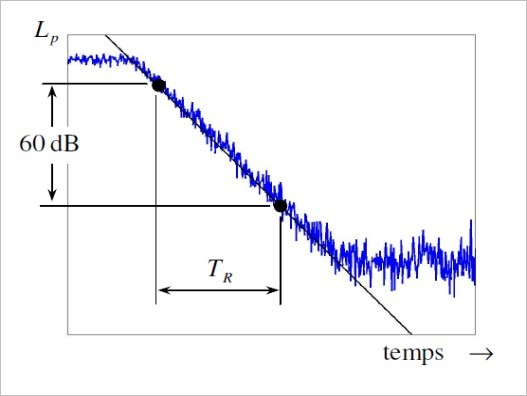
\includegraphics[scale=.3]{graph/reverberationtime}%
    \end{figure}
    \addreference{\href{http://vibroacoustique.fr/cours/M03_C01/co/grain05.html}{vibroacoustique.fr/cours/M03\_C01/co/grain05.html}}
    \question{what are typical ranges for the room reverberation times}
    
    \begin{itemize}
        \item \unit[0.2-10]{s}
    \end{itemize}
\end{frame}

\begin{frame}{artificial reverberation}{room simulation: ray tracing}
	\begin{figure}
		\centerline{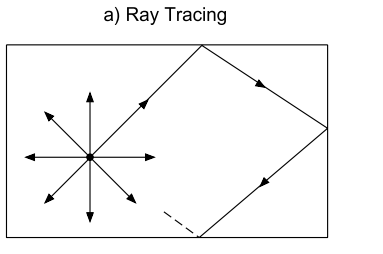
\includegraphics[scale=.4]{graph/raummodell1}}
	\end{figure}
	\begin{figure}
		\centerline{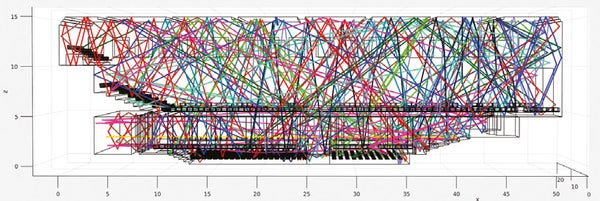
\includegraphics[scale=.4]{graph/raytracing}}
	\end{figure}
    
    \addreference{\href{https://issuu.com/epccedinburgh/docs/epcc_news_83/s/5015}{issuu.com/epccedinburgh/docs/epcc\_news\_83/s/5015}}
    
\end{frame}

\begin{frame}{artificial reverberation}{room simulation: mirror model}
    \vspace{-3mm}
	\begin{figure}
		\centerline{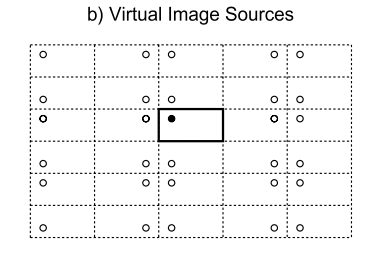
\includegraphics[scale=.4]{graph/raummodell2}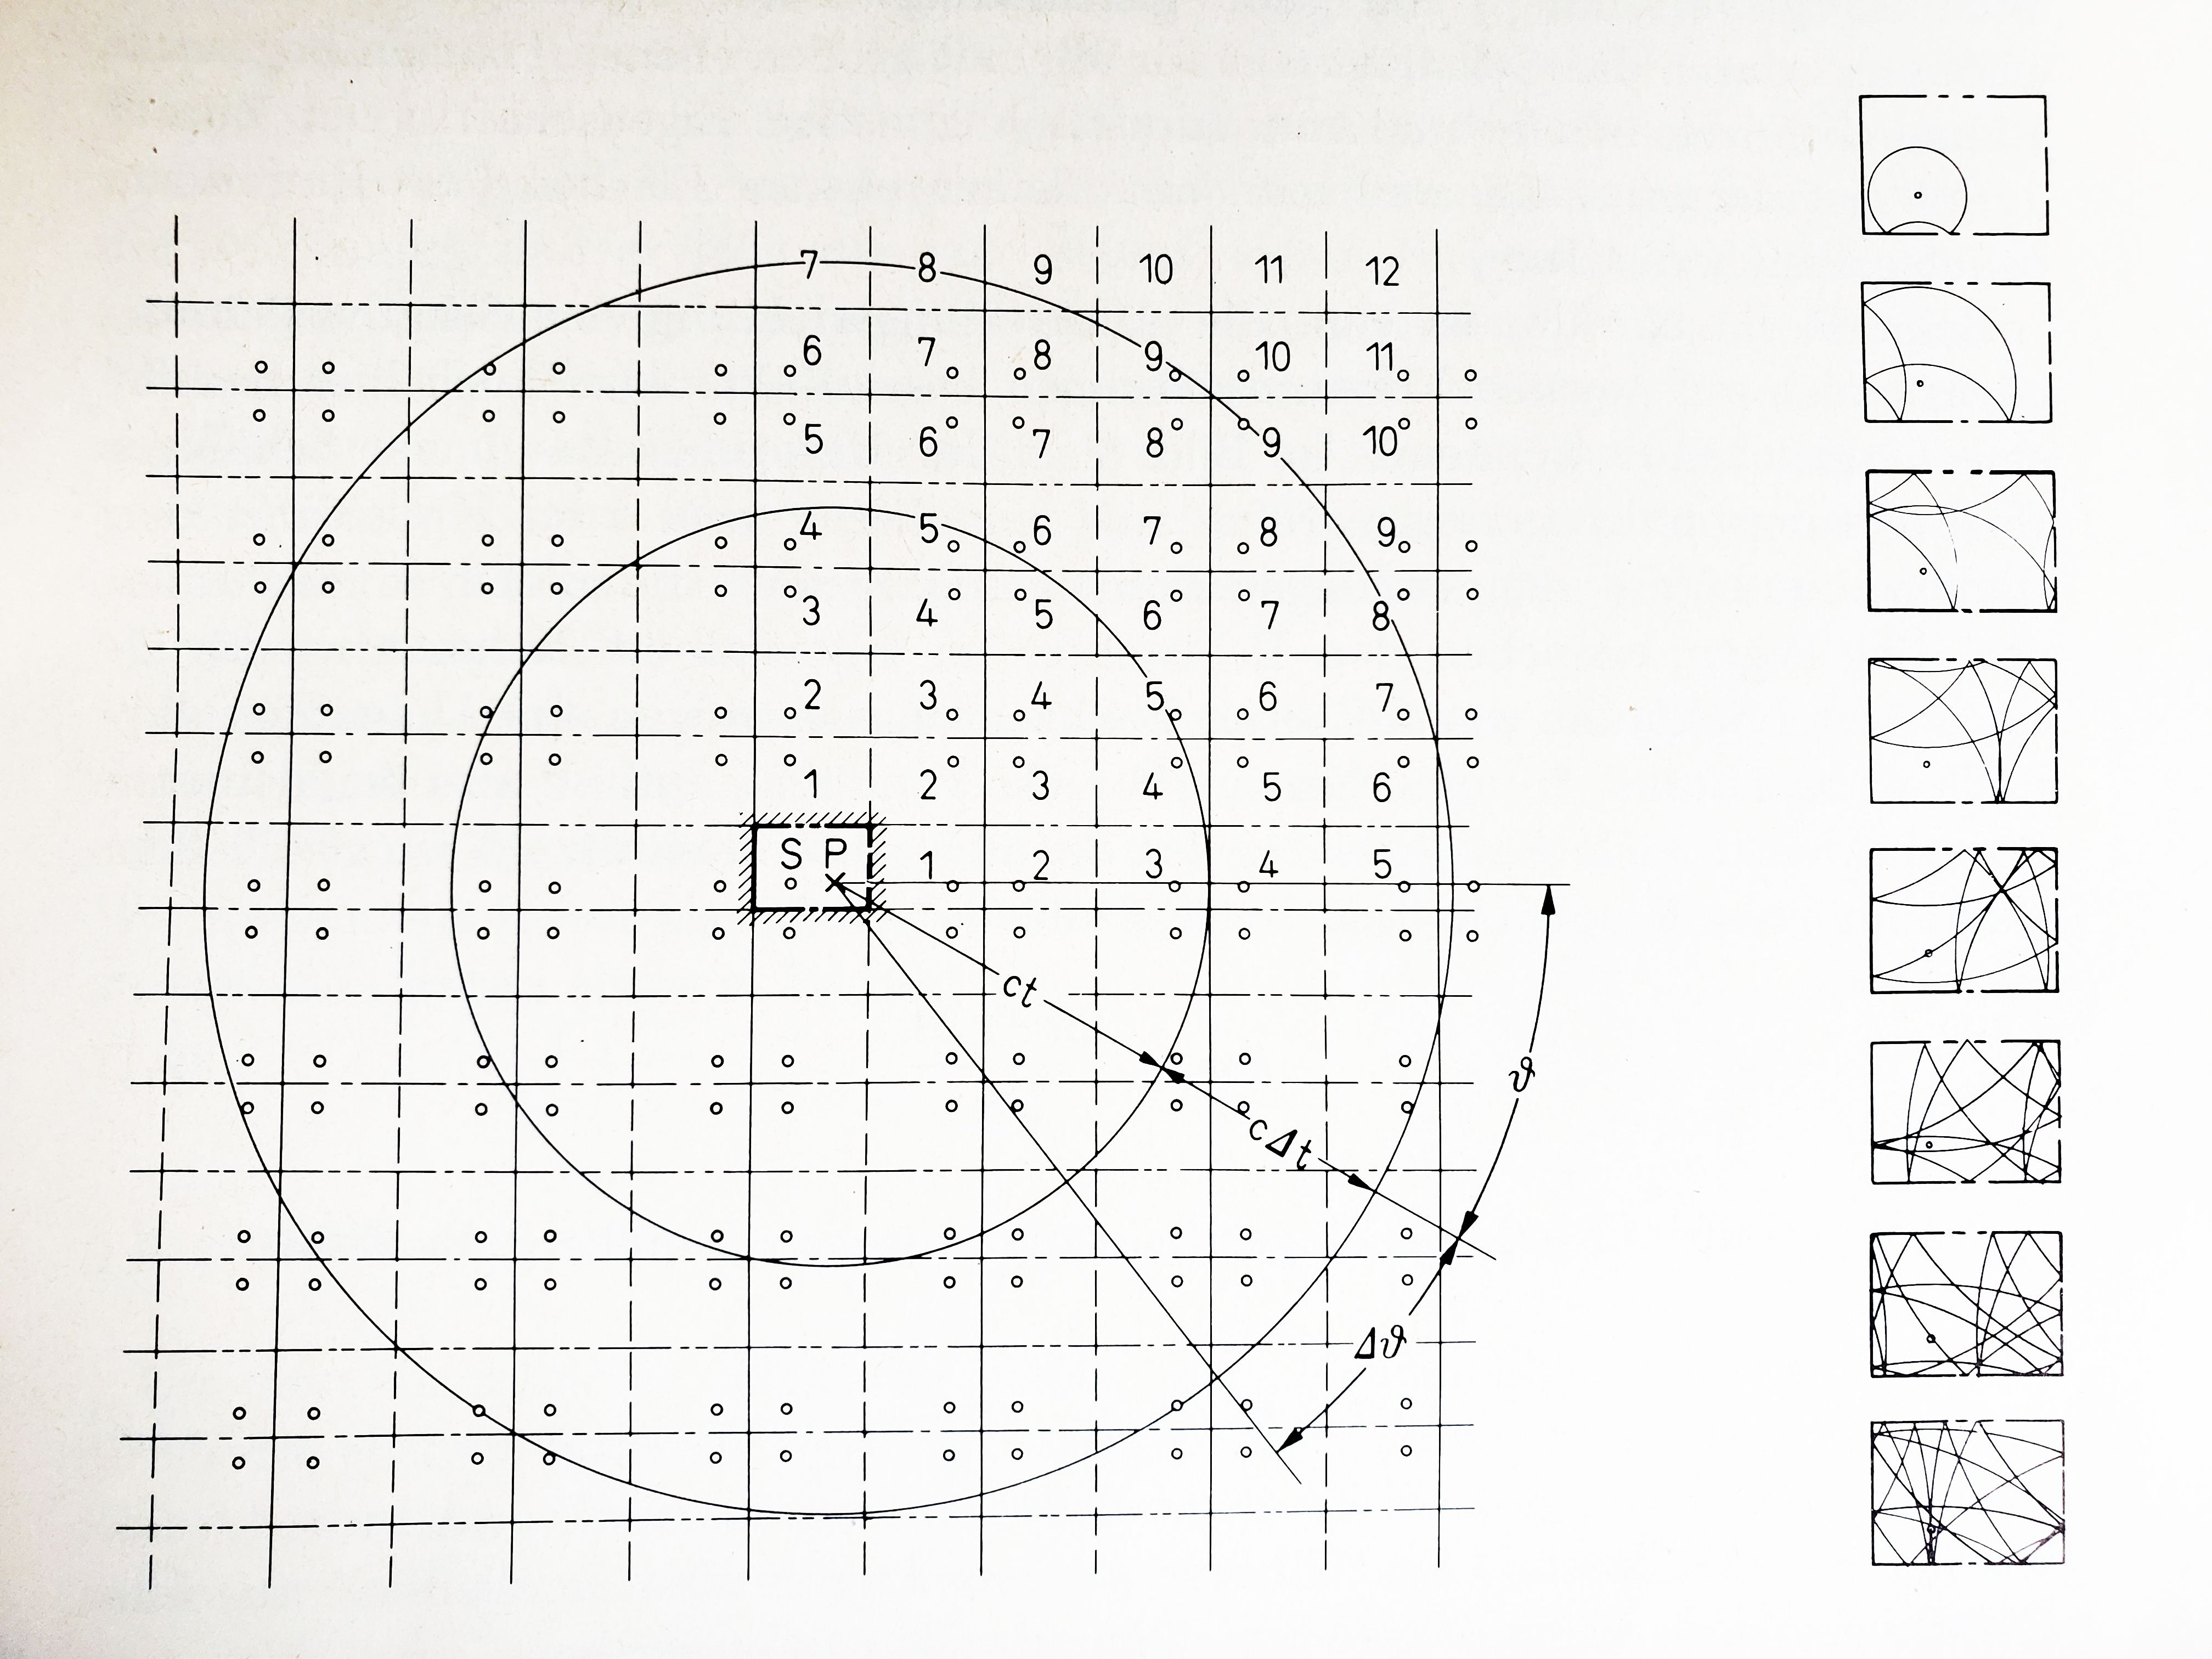
\includegraphics[scale=.05]{graph/mirrormodel}}
		%\centerline{}
	\end{figure}
    
    \phantom{\footfullcite{cremer_wissenschaftlichen_1978}}
    \vspace{-3mm}
    
\end{frame}

\section{artificial reverb}
\begin{frame}{artificial reverberation}{convolution vs.\ parametric reverb}
    \begin{itemize}
        \item   \textbf{convolution reverb}
            \begin{itemize}
                \item[+]   IR measured or generated by model
                \item[+]   realistic
                \item[--]  restriction to pre-generated IR libraries
                \item[--]  high workload and memory requirements
            \end{itemize}
        \bigskip
        \item   \textbf{parametric reverb}
            \begin{itemize}
                \item[+]   can be very efficient
                \item[+]   can be parametrized
                \item[--]  less realistic/no real-world IRs
            \end{itemize}
    \end{itemize}
\end{frame}

%\section{components}
\begin{frame}{artificial reverberation}{traditionally used filters: comb filter}
	        \begin{figure}
				\begin{center}
	            \begin{picture}(50,30)
	
	                %boxes
	                \put(25,5){\framebox(7,6){\footnotesize{$z^{-N}$}}}
	
	                %lines horizontal
	                \put(0,20){\vector(1,0){14}}
	                \put(16,20){\vector(1,0){32}}
	                \put(50,20){\vector(1,0){5}}
	                
	                \put(15,8){\line(1,0){10}}
	                \put(42,8){\vector(-1,0){10}}
	
	                %lines vertical
	                \put(42,20){\line(0,-1){12}}
	                \put(15,8){\vector(0,1){4}}
	                \put(15,14){\vector(0,1){5}}
	                
	                %circles
	                \put(47.5,19){$\otimes$}
	                \put(13.5,19){$\oplus$} % 15-20
	                \put(13.5,12){$\otimes$}
	                
	                \put(42,20){\circle*{1}}
	
	                %text
	                \put(43,22){\footnotesize{\shortstack[c]{$b_0$}}}
	                \put(8,10){\footnotesize{\shortstack[c]{$-a_N$}}}
	
	                \put(-2,22){\footnotesize{\shortstack[c]{x(n)}}}
	                \put(52,22){\footnotesize{\shortstack[c]{y(n)}}}
	
	            \end{picture}
				\end{center}
	        \end{figure}
        	\begin{eqnarray*}
        		y(n) &=& b_0\cdot x(n) - a_N\cdot y(n-N)\\
	    		H(z) &=& \frac{b_0}{1-a_N\cdot z^{-N}}
        	\end{eqnarray*}
\end{frame}
\begin{frame}{artificial reverberation}{traditionally used filters: all pass filter}
		    \begin{figure}
				\begin{center}
		        \begin{picture}(30,40)
		
		            %boxes
		            \put(11,21){\framebox(8,8){\footnotesize{$z^{-M}$}}}
		
				
		            %lines horizontal
		            \put(0,25){\vector(1,0){11}}
		            \put(19,25){\vector(1,0){10}}
		
		            \put(31,25){\vector(1,0){4}}
		            \put(5,35){\vector(1,0){9}}
		            \put(16,35){\line(1,0){14}}
		            
		            \put(0,15){\line(1,0){14}}
		            \put(25,15){\vector(-1,0){9}}
		            \put(-5,25){\vector(1,0){4}}
		            
		            %lines vertical
		            \put(5,25){\line(0,1){10}}
		            \put(30,35){\line(0,-1){9}}
		            
		            \put(0,15){\vector(0,1){9}}
		            \put(25,25){\line(0,-1){10}}
		            
		            %circles
		            \put(13.5,34){$\otimes$} %15,35
		            \put(28.5,24){$\oplus$} % 30,25
		            \put(13.5,14){$\otimes$} % 
		            \put(-1.5,24){$\oplus$} % 0,25
		            
		            \put(5,25){\circle*{1}}
		            \put(25,25){\circle*{1}}
		
		            %text
		            \put(-5,28){\footnotesize{\shortstack[c]{x(n)}}}
		            \put(35,28){\footnotesize{\shortstack[c]{y(n)}}}
		            \put(16,36){\footnotesize{\shortstack[c]{g}}}
		            \put(16,12){\footnotesize{\shortstack[c]{-g}}}
		
		        \end{picture}
				\end{center}
		    \end{figure}
			\begin{eqnarray*}
				y(n) &=& g\cdot x(n) + x(n-M) - g\cdot y(n-M)\\
				H(z) &=& \frac{z^{-M} + g}{1 + g\cdot z^{-M}}
			\end{eqnarray*}
\end{frame}

\section{Schroeder}
\begin{frame}{artificial reverberation}{reverberation: Schroeder 1/2}
		\begin{figure}
			\centerline{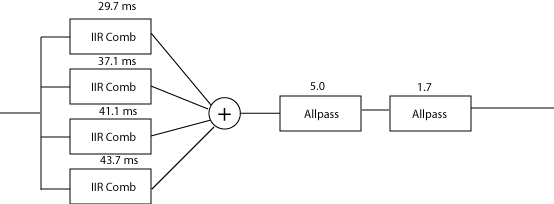
\includegraphics[scale=.5]{graph/schroeder}}
		\end{figure}     
        \phantom{\footfullcite{schroeder_colorless_1961}}
		%\vspace{-3mm}
		\pause
		\textbf{questions}:
        \smallskip
		
        \begin{itemize}
			\item	how to change the reverberation time?
			\item	how to change the density?
		\end{itemize}
\end{frame}

\begin{frame}{artificial reverberation}{reverberation: Schroeder 2/2}
    \begin{itemize}
        \item   \textbf{problems}
            \begin{itemize}
                \item	sound coloring ($\rightarrow$ prime numbers)
                \item	periodicity
            \end{itemize}
        \pause
        \bigskip
        \item   \textbf{audio}
            \begin{itemize}
                \item   original \includeaudio{sv}
                \item   wet \includeaudio{svRevSchroeder}
            \end{itemize}
    \end{itemize}
\end{frame}

\section{other}
\begin{frame}{artificial reverberation}{reverberation: Moorer}
    \vspace{-5mm}
    \begin{columns}
    \column{.5\linewidth}
	\begin{itemize}
		\item	similar to Schroeder's model
		\item	more comb filters
		\item	low pass in feedback paths
		\item	simple FIR model for early reflections
	\end{itemize}
    \column{.5\linewidth}
        \begin{figure}
            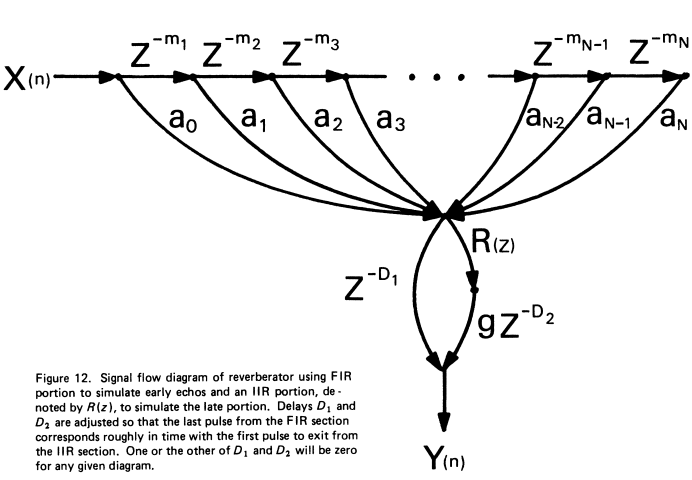
\includegraphics[scale=.3]{graph/moorer}
        \end{figure}
    \end{columns}
    \begin{itemize}
        \item   original \includeaudio{sv}
        \item   wet \includeaudio{svRevMoorer}
    \end{itemize}
        \phantom{\footfullcite{moorer_about_1979}}
\end{frame}

\begin{frame}{artificial reverberation}{other reverberation approaches: Gardner}
	\begin{figure}
		\centerline{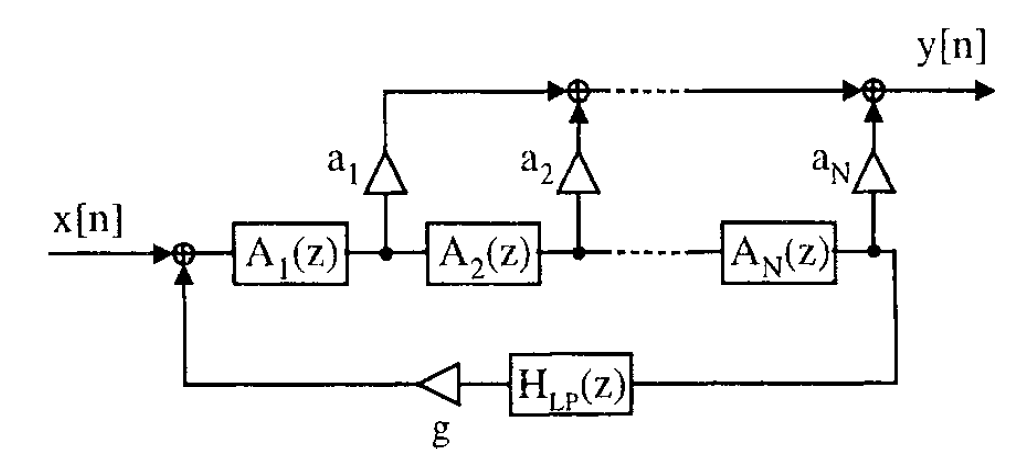
\includegraphics[scale=.4]{graph/gardnerreverb}}
	\end{figure} 
\end{frame}

\begin{frame}{artificial reverberation}{other reverberation approaches: Jot (feedback delay network)}
	\begin{figure}
		\centerline{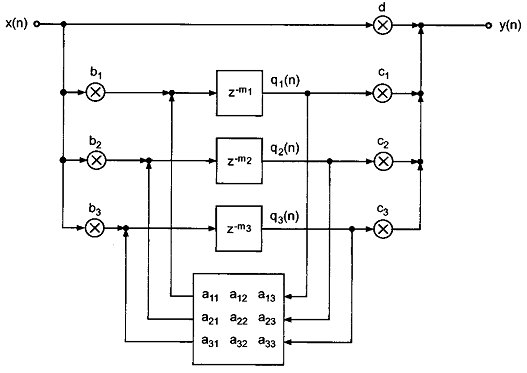
\includegraphics[scale=.5]{graph/fdn}}
	\end{figure} 
\end{frame}

\section{Dattorro}
\begin{frame}{artificial reverberation}{reverberation: Dattorro 1/2}
	\vspace{-6mm}
    \framezoom<1><2>[border](1.9cm,-.5cm)(6.8cm,3.5cm)
    \framezoom<1><3>[border](1.9cm,3cm)(6.8cm,4.5cm)
    \begin{figure}
		\centerline{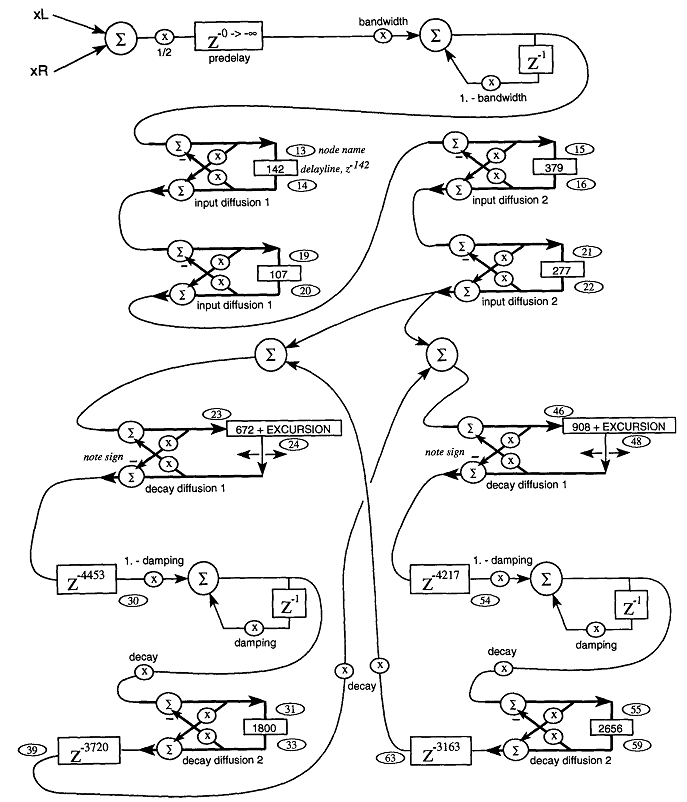
\includegraphics[scale=.37]{graph/dattorro}}
	\end{figure} 
    \phantom{\footfullcite{dattorro_effect_1997a}}    
\end{frame}

\begin{frame}{artificial reverberation}{reverberation: Dattorro 2/2}
	intention: plate reverb model \pause (dense, bright, fast build-up time)
    \bigskip
    \begin{itemize}
        \item   original \includeaudio{sv}
        \item   wet (Plate) \includeaudio{svRevDattorroPlate}
        \item   wet (Medium Hall) \includeaudio{svRevDattorroMedHall}
        \item   wet (Cathedral) \includeaudio{svRevDattorroCathed}
    \end{itemize}
\end{frame}

\section{early reflections}
\begin{frame}{artificial reverberation}{early reflections: models 1/2}
	\begin{figure}
		\centerline{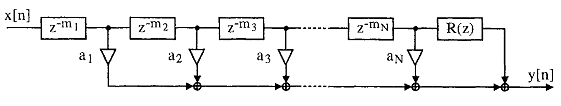
\includegraphics[scale=.6]{graph/er_simple}}
	\end{figure}
\end{frame}

\begin{frame}{artificial reverberation}{early reflections: models 2/2}
	\begin{figure}
		\centerline{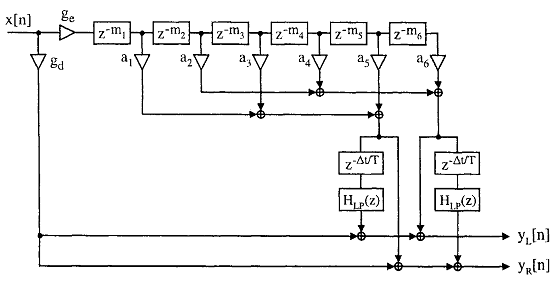
\includegraphics[scale=.6]{graph/erstandard}}
	\end{figure}
\end{frame}

\section{implementation}
\begin{frame}{artificial reverberation}{quality enhancements}
	\begin{itemize}
		\item	\textbf{multi-channel processing}
			\begin{itemize}
				\item	mono in $\rightarrow$ mono out				
				\item	mono in $\rightarrow$ stereo out				
				\item	stereo in $\rightarrow$ stereo out
			\end{itemize}
		\pause
        \bigskip
		\item	\textbf{delay modulation}
			\begin{itemize}
				\item	increase ``diffusity'' and ``liveliness''
			\end{itemize}
	\end{itemize}
\end{frame}

\begin{frame}{artificial reverberation}{common parameters}
	\begin{itemize}
		\item	wetness
		\pause
		\item	reverberation time
		\pause
		\item	pre-delay
		\pause
		\item	low pass cutoff
		\pause
		\item	low pass slope
		\pause
		\item	bass boost
		\pause
		\item	ratio of early reflection/late reverberation
		\pause
		\item	diffusion, liveliness, etc.
	\end{itemize}
\end{frame}

	
\section{summary}
		\begin{frame}{summary}{parametric reverb}
            \begin{itemize}
                \item \textbf{advantages} over convolution reverbs
                    \begin{itemize}
                        \item   fully parametrizable --- not restricted to predefined IR library
                        \item   works well with already somewhat reverberated recordings 
                        \item   lower workload (IIR vs.\ FIR)
                    \end{itemize}
                \bigskip
                \item<2-> \textbf{disadvantages} over convolution reverbs
                    \begin{itemize}
                        \item   less realistic, no real-world IRs
                    \end{itemize}
            \end{itemize}
 		\end{frame}

\end{document}

